\documentclass[11pt]{article}
\usepackage[margin=1in]{geometry}
\usepackage[textsize=footnotesize, backgroundcolor=white]{todonotes}
\usepackage[T1]{fontenc}
\usepackage[utf8]{inputenc}
\usepackage{amsmath}
\usepackage{natbib}
\usepackage{titling}

\begin{document}

%---------------------------------------------
%---------------------------------------------
\section*{A bayesian method for the evaluation of a trait-matching model}

We are interested to evaluate from empirical data a function describing the probability of an interaction between species $i$ and $j$ based on their respective sets of traits $\mathbf{T}_i$ and $\mathbf{T}_j$. It has been found that most interactions could be represented within a trait space (Eklof et al. 2013 - Fig. 1A) that has from 3 - 5 dimensions. The challenge is to fit a statistical model that will relate the probability an interaction occurs to the set of traits of the two species. For instance, we might want to fit the model giving the probability a predator of size $M_{pred}$ feeds on a prey of size $M_{prey}$ (e.g. Gravel2013). 

More specifically, for a given set of traits $1$ and $2$, we are looking for:

\begin{equation}  
	P(L_{ij}=1|T_{i1},T_{j2})
\end{equation}

Which reads as the probability of observing an interaction $L$ between species $i$ and $j$ given the traits $T_{i1}$ and $T_{j2}$. The function describing this probability could take any form. For the sake of the example here we will consider a gaussian function to represent the interaction niche (Williams2010, see below) but other functions, such as high order polynomial or even regression trees, could be considered as well. The gaussian function is however convenient because easy to integrate, while other ones might not and thus could require more complicated fitting algorithms such as MCMC. 

Equation 1 could be used as a likelihood function that we want to fit directly to empirical data. To do so, the required data should contain information about the set of traits for the two nodes (e.g. a consumer and a resource, or a plant and a pollinator), and the observation of presence and absence of interactions. For instance, the matching-centrality algorithm (Rohr and Bersion, 2010) evaluates a binomial model representing the interaction probability as a function of the squared difference between traits of the consumer and the resource. The problem we are facing however is that records of the absence of interactions are often not available in most datasets of ecological interactions, except for network data. In other words, we have data only for the black dots at Fig. 1A, but not for the white dots, thus preventing us to draw the borders of the interaction niche. Alternatively, there might be considerable uncertainty in the absence of interactions (false negatives). One could always argue that if two species are not found interacting they will never do so. But there could be sampling issues since one (or both) species could be extremely rare, making the likelihood of an interaction very low. In this situation, any record of an absent interaction would be highly sensitive to sampling intensity. Alternatively, the species could not be found in the same geographic area and consequently we would have no information about their capability to interact. The latter issue will be common for datasets compiled at very large spatial scale.  Such absence of interactions does not imply they will not interact in the future, neither there is a trait matching constraint preventing their interaction. We therefore present a bayesian methodology to fit Eq. 1 indirectly, using only information about the observed interactions. 

Presence only data has information about the traits of species $i$, of species $j$ and the interaction $L_{ij} = 1$. We consequently revise the problem and model the probability of sampling trait $T_{i1}$: 

\begin{equation}  
	P(T_{i1}|L_{ij}=1,T_{j2})
\end{equation}

Which could interpreted as \emph{the probability that we sample trait $T_{i1}$ given we know there is an interaction between species $i$ and $j$ and the trait $T_{j2}$}. This equation provides the likelihood for any observation of an interaction based on traits of the two species. We now use Bayes' theorem $p(A|B)p(B) = p(B|A)p(A)$ to decompose Eq. 2, yielding the following function: 

\begin{equation}  
	P(T_{i1}|L_{ij}=1,T_{j2})=\frac{P(L_{ij}=1|T_{i1},T_{j2})P(T_{i1})}{P(L_{ij}=1|T_{j2})}
\end{equation}

$P(T_{i1}$ is the probability density function for the trait $T_{i1}$. It corresponds to the frequency of this trait in the regional pool. It could thus be weighted by abundance (see below in the \textbf{Neutral} subsection). The denominator is the marginal distribution of the interaction probability, computed as the integral of the numerator over the whole distribution of the trait $T_{i1}$:

\begin{equation}  
	P(L_{ij}=1|T_{j2})=\int_{-\infty}^{\infty}P(L_{ij}=1|T_{i1},T_{j2})P(T_{i1})dT_{i1}
\end{equation}

The overall principle of the method is best interpeted in light of Fig 1B. Take for instance the case of a predatory fish species of size $M_{pred}$ sampling the distribution of body mass of a set of preys, $P(M_{preys})$. We know that larger fish typically feed on smaller fish species because they require the prey fitting their mouth. The frequency distribution of prey size will indeed influence the distribution of the body mass in the diet of the predator, even if the predator has a preferred prey size. The predator does not sample that distribution randomly however, but rather it targets only a specific range (given by Eq.1). Both the available prey distribution ($P(M_{prey}$) and the posterior prey distribution ($P(M_{prey} |L,M_{pred}$) are illustrated at Fig. 1B. The posterior prey distribution will be somewhere in between the regional prey distribution, and its niche. The model therefore integrates both neutral and trait-matching constraints. 

As a side product, the denominator informs us of the generality of the consumer. This integral might be tricky to compute analytically, depending on the form of Eq. 1 and the type of distribution, but most software nowadays offer easy ways to compute it numerically. Here the usage of the gaussian function simplifies computations. 

We provide an example at Fig 1C for trophic interactions in marine systems. We use data from Barnes et al. (2008), using log body size for predator ($M_{pred}$) and the prey ($M_{prey}$). The trait-matching function is based on the niche model (Williams2000), where the main niche axis is the log of body size. In this situation, both $T_1$ and $T_2$ are the same trait. The log body size of the predator determines its optimum and the range of its niche, while the log prey size its niche position (Gravel et al. 2013). We consider a gaussian function to represent the probability of an interaction given the size of the predator and the prey:

\begin{equation}  
	P(L_{ij}=1|M_{pred},M_{prey})= exp\frac{-(\alpha_0+\alpha_1*M_{pred}-M_prey)^2}{2(\beta_0+\beta_1*M_{pred})^2}
\end{equation}

Where $\alpha_0$, $\alpha_1$, $\beta_0$ and $\beta_1$ are fitted parameters describing the linear relationship between the predator size, its optimum and the range of its niche (other shapes could be used as well). One tricky issue might be to gather information about the trait distribution. We assume the distribution of the data provides a decent representation of the distribution of potential prey sizes. One could take the moments of the trait distribution at the species level or at the individual level. We consider a normal distribution for the log of prey body size. The Fig 1C represents the data and the best fit model (all of the code necessary to perform this analysis is provided in the supplementary material). 

\subsection*{Pure neutral interactions}

The above model integrates both trait-matching and abundance constraints. The model could be simplified to account only for the effect of abundance (trait distribution) to reveal the importance of the trait-matching constraint. Previous analyses have shown that interaction networks are significantly impact by abundance distribution (REFS). The structure of interaction networks could be reasonnably approximated with a neutral model (REFS). A neutral model in this framework is found when the probability of an interaction is equally probable, irrespective of the traits of the two species involved in the interaction. In other words, $P(L_{ij}=1|T_{iA},T_{jB})=k$. In this situation, the probability of sampling trait $T_{i1}$ is given by: 

\begin{equation}  
	P(T_{i1}|L_{ij}=1,T_{j2})=\frac{kP(T_{i1})}{\int_{-\infty}^{\infty}kP(T_{i1})dT_{i1}}
\end{equation}

Which reduces to the distribution $P(T_{i1})$ because the integral of the PDF sums to 1 by definition, and the simplification of the constant $k$. 

\subsection*{Pure niche interactions}

Alternatively, one could want to compare to the situation where interactions are purely determined by trait-matching constraints. In this situation, we consider the distribution of the trait $T_1$ to be uniform within the range of the observed traits. The probability of sampling trait $T_{i1}$ in this situation is by definition $1/(max(T_{i1})-min(T_{i1}))$, for all trait values. The denominator simplifies to the integral of the gaussian function (Eq. 5), $r\sqrt{2\pi}$, and thus the posterior distribution of the pure niche model takes the form: 

\begin{equation}  
	P(T_{i1}|L_{ij}=1,T_{j2})=\frac{P(L_{ij}=1|T_{i1},T_{j2})}{(max(T_{i1})-min(T_{i1}))r\sqrt{2\pi}}
\end{equation}

\subsection*{Multi-trait expansion}

The extension to multiple trait matching contraints is straightforward to perform. It requires assuming that the different trait matching functions are independent (cases of non-independence are possible but beyond the scope of the current paper). Because of this assumption, the joint probability is easily expanded using the relationship $P(x,y) = P(x)P(y)$:

\begin{equation}  
	P(T_{i1},T_{i3}|L_{ij}=1,T_{j2}T_{j4})=\frac{P(L_{ij}=1|T_{i1},T_{j2})P(T_{i1})}{P(L_{ij}=1|T_{j2})}\frac{P(L_{ij}=1|T_{i3},T_{j4})P(T_{i3})}{P(L_{ij}=1|T_{j4})}
\end{equation}

\begin{figure} 
\centering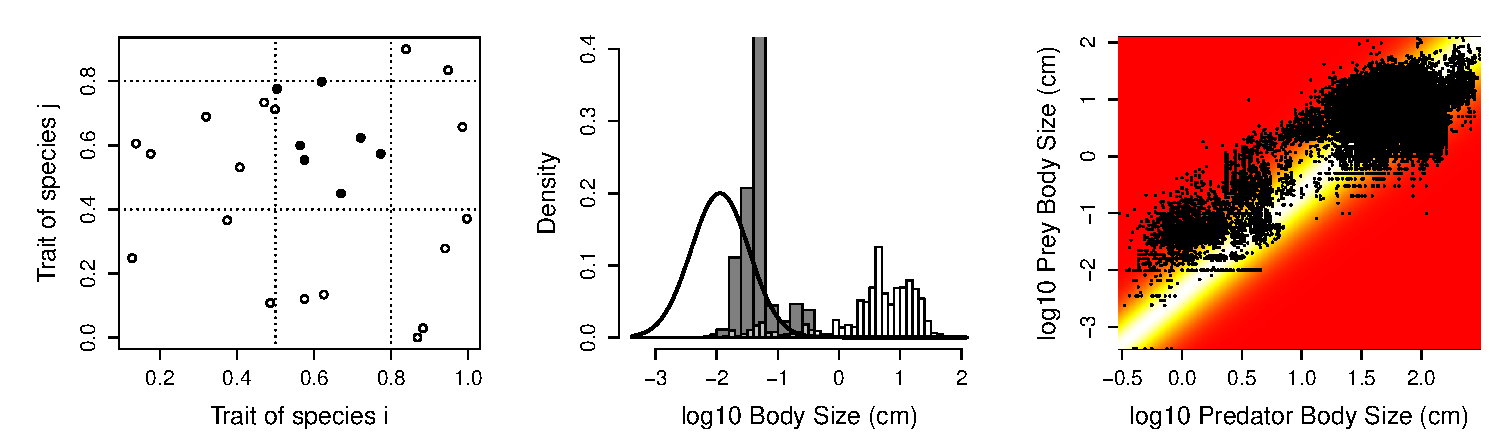
\includegraphics[width=0.9\textwidth]{fig_box2.pdf}
\caption{Illustration of the quantitative framework to evaluate a trait-matching function. A) Conceptual representation of a trait-matching constraint. Interactions (in black) are observed only when both species have traits that are compatible. B) Representation of the density function for available body size in the Barnes et al. (2008) dataset, the trait-matching function (red line) and the observed distribution of prey size for a given predator (black lines). C) Representation of the observed interactions (black dots) and the maximum likelihood estimate of the trait-matching function (from low probability in yellow to high probability in red). }
\end{figure}

\end{document}














